\newpage
\section{Ascending delay function: Delay of 6}

\begin{figure}[hb]
 %   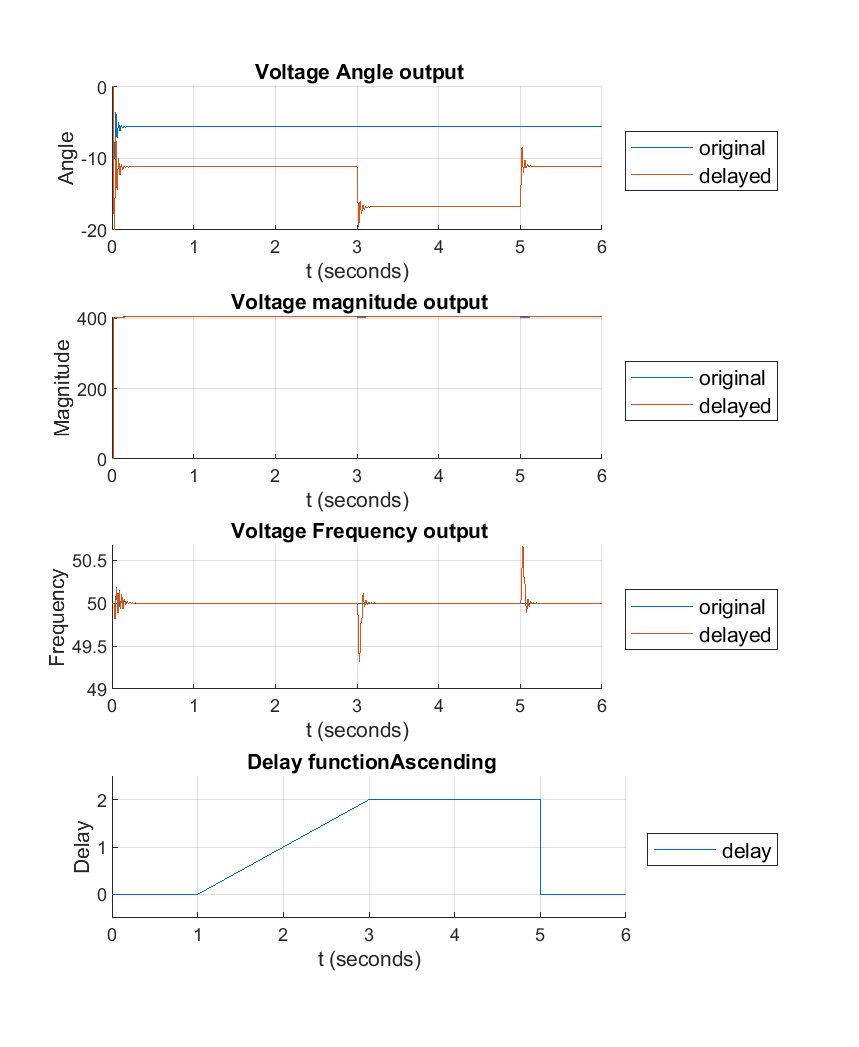
\includegraphics[trim=2 10 14 4, clip]{figures/v_AllFig-DelayOf_2-Ascending.png}    
    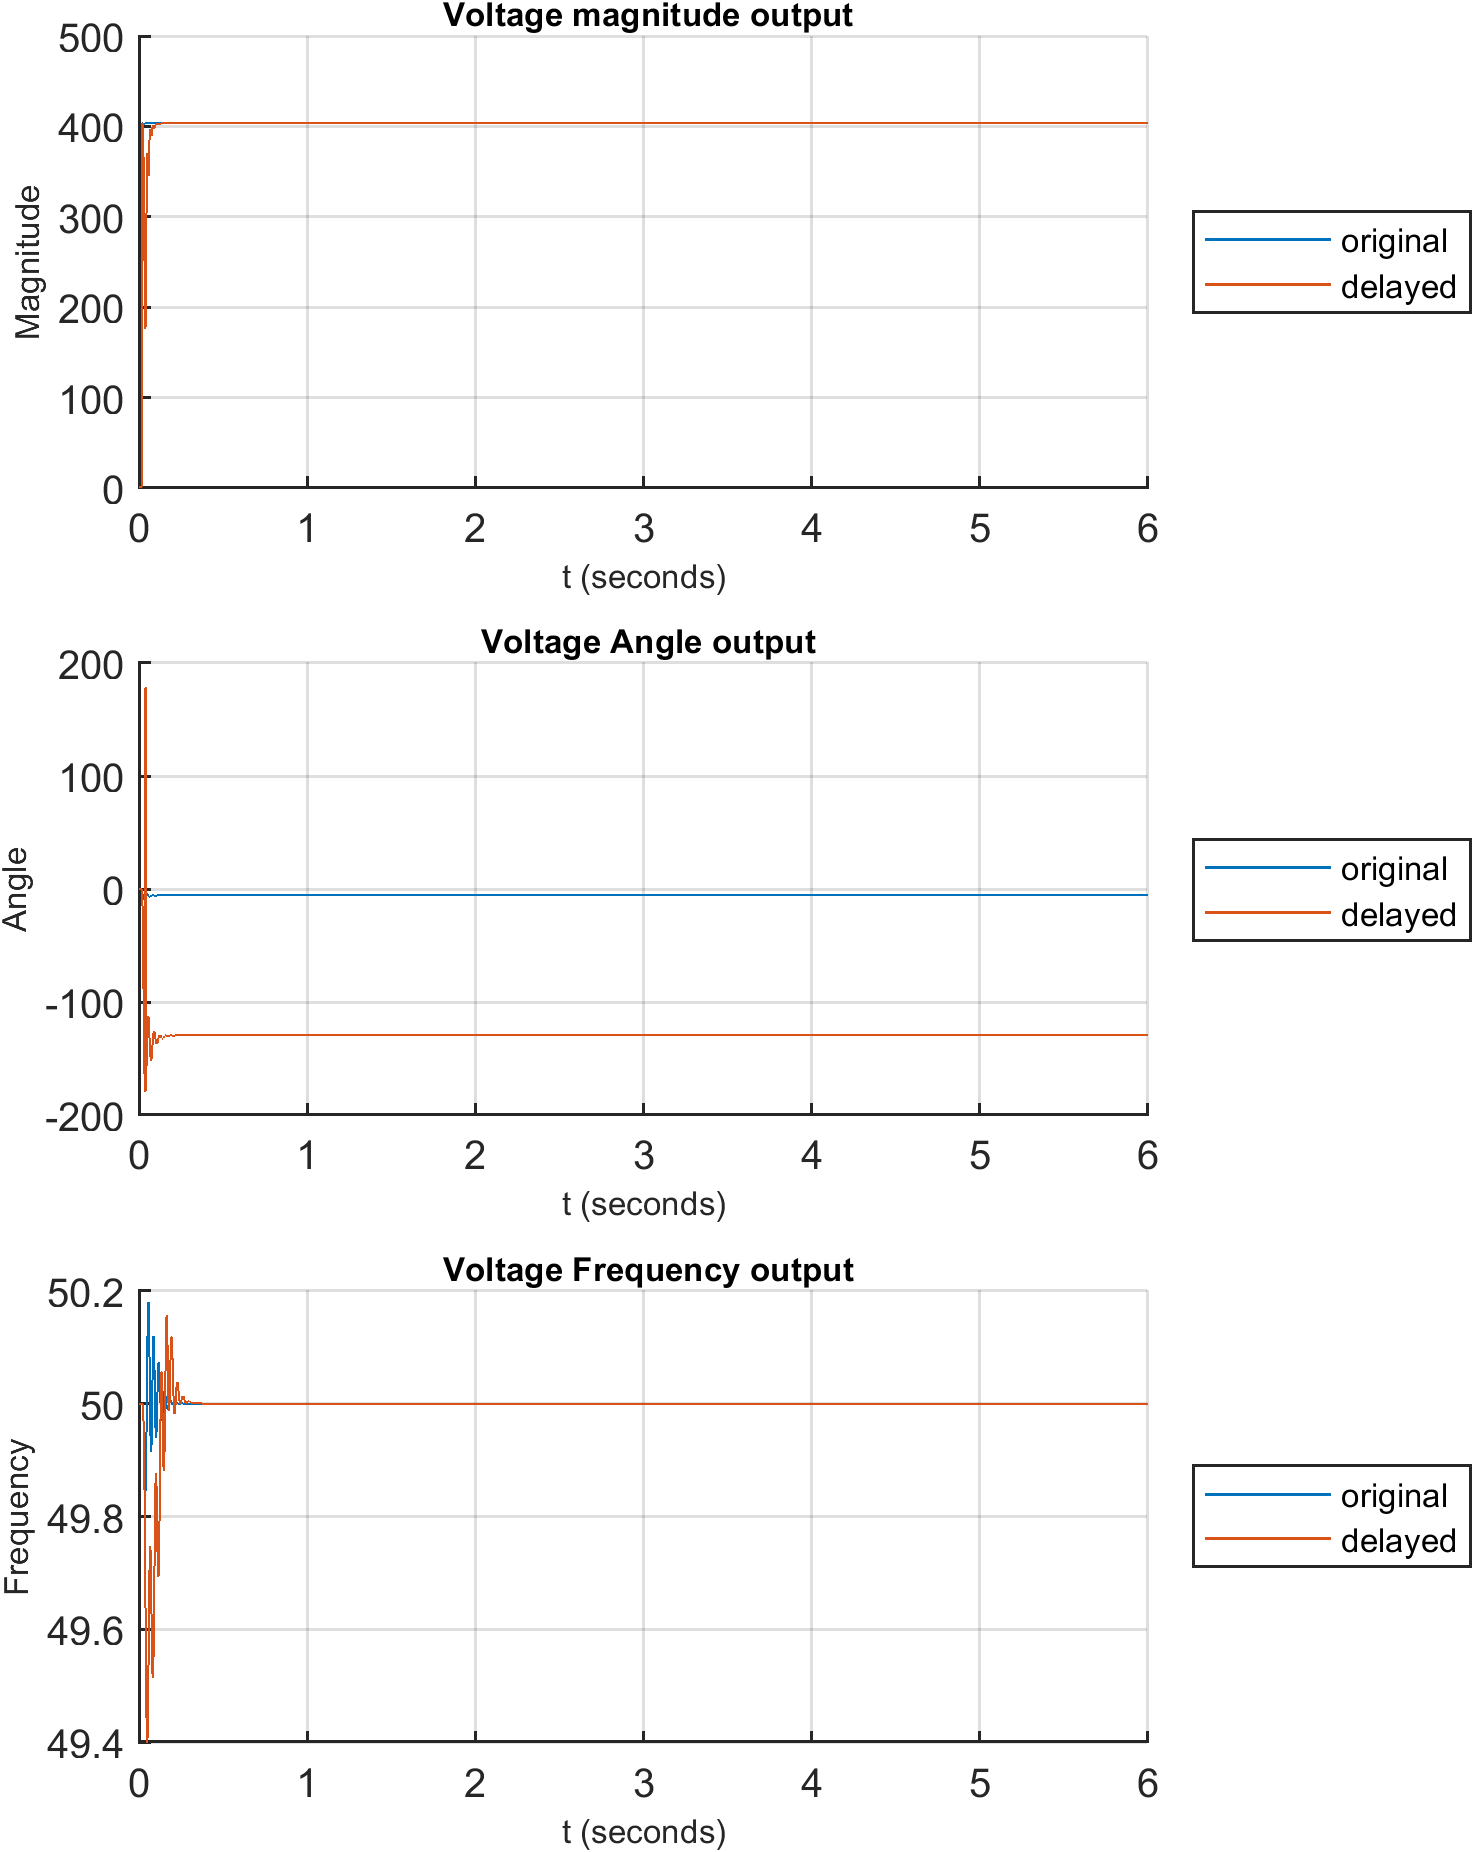
\includegraphics[width=0.95\textwidth]{\locateResults/AllFig.png}    
    \caption{Ascending delay of 6: Combined output}
    \label{fig:PMUsim-Con6-allfig}
\end{figure}


     \begin{figure}
 
    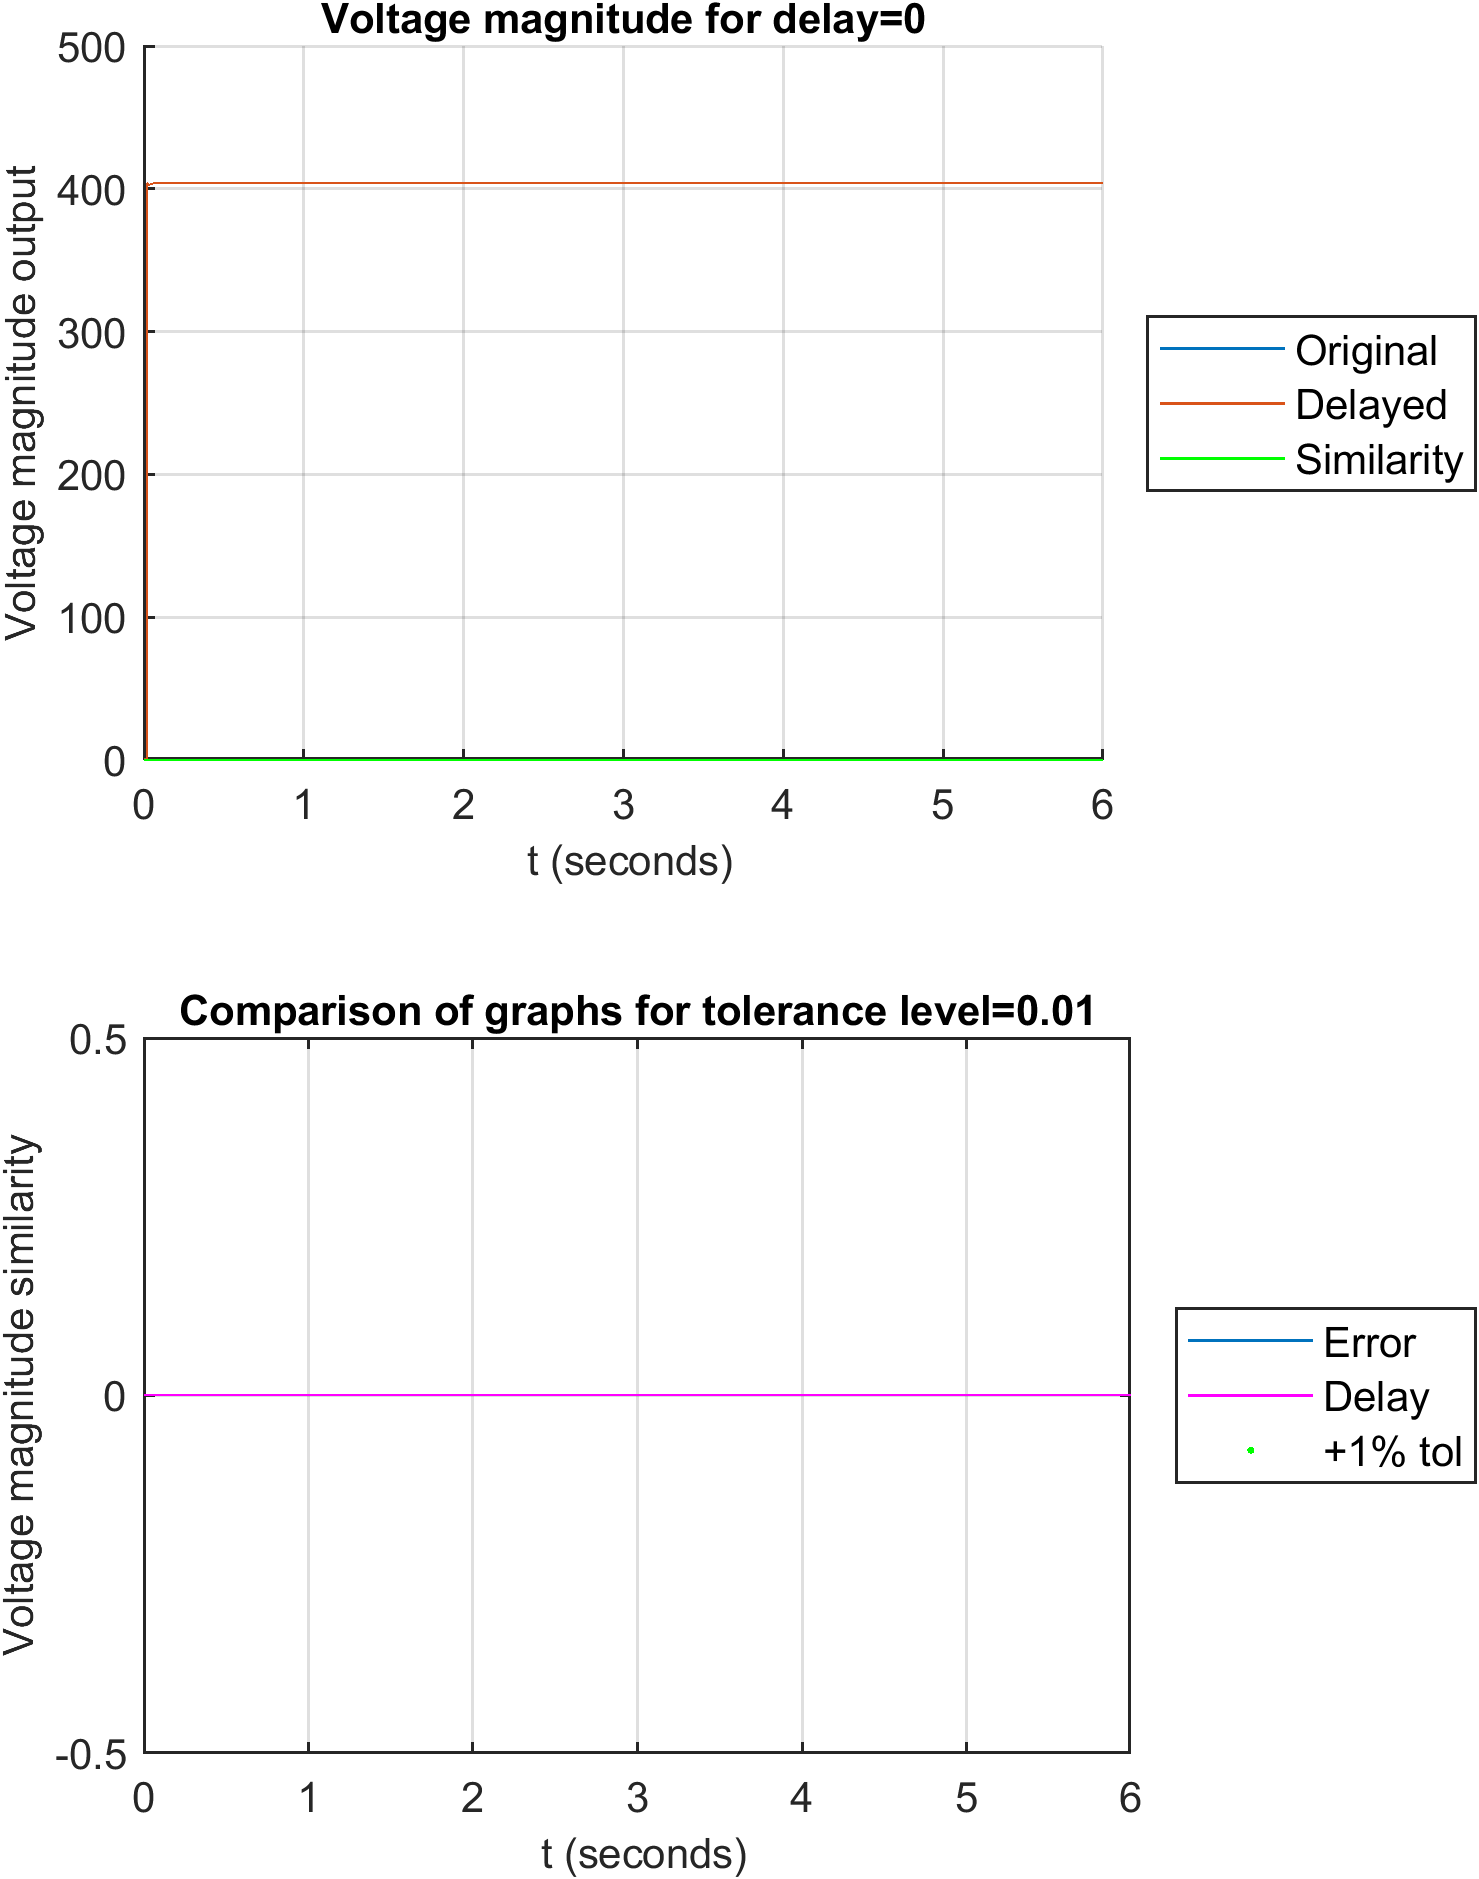
\includegraphics[width=\textwidth]{\locateResults/Magnitude.png}    
         %\caption{magnitude Output}
         \label{fig:PMUsim-Con6Mag}
        \caption{Ascending delay of 6: Magnitude component output}
 
\end{figure}

     \begin{figure}
 
   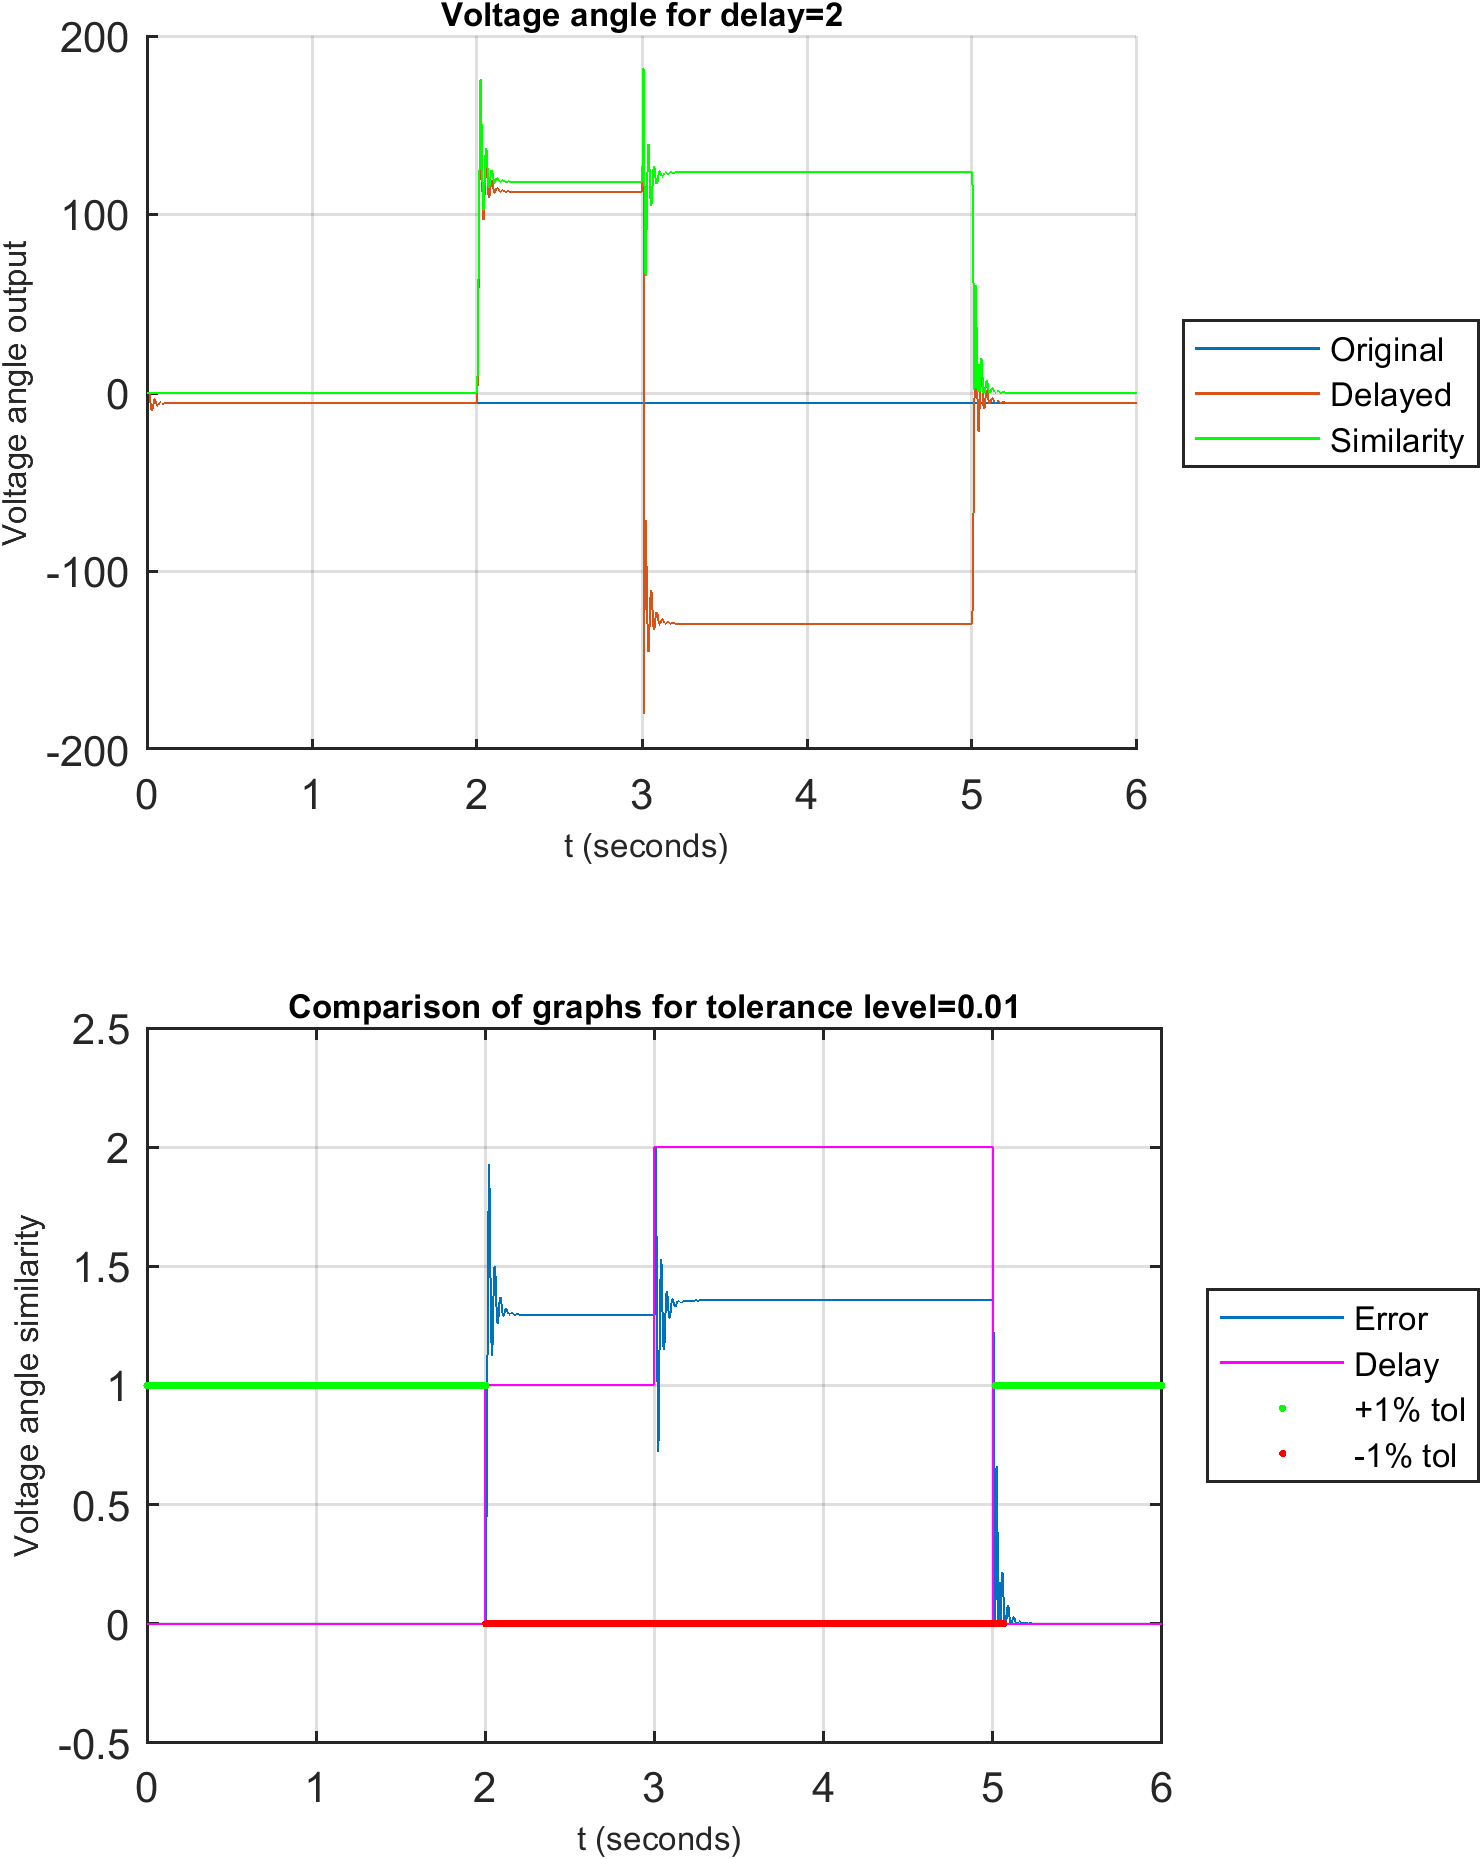
\includegraphics[width=\textwidth]{\locateResults/Angle.png}    
          %\caption{Angle Output}
         \label{fig:PMUsim-Con6Ang}
        \caption{Angle component output}
 
\end{figure}

     \begin{figure}
 
   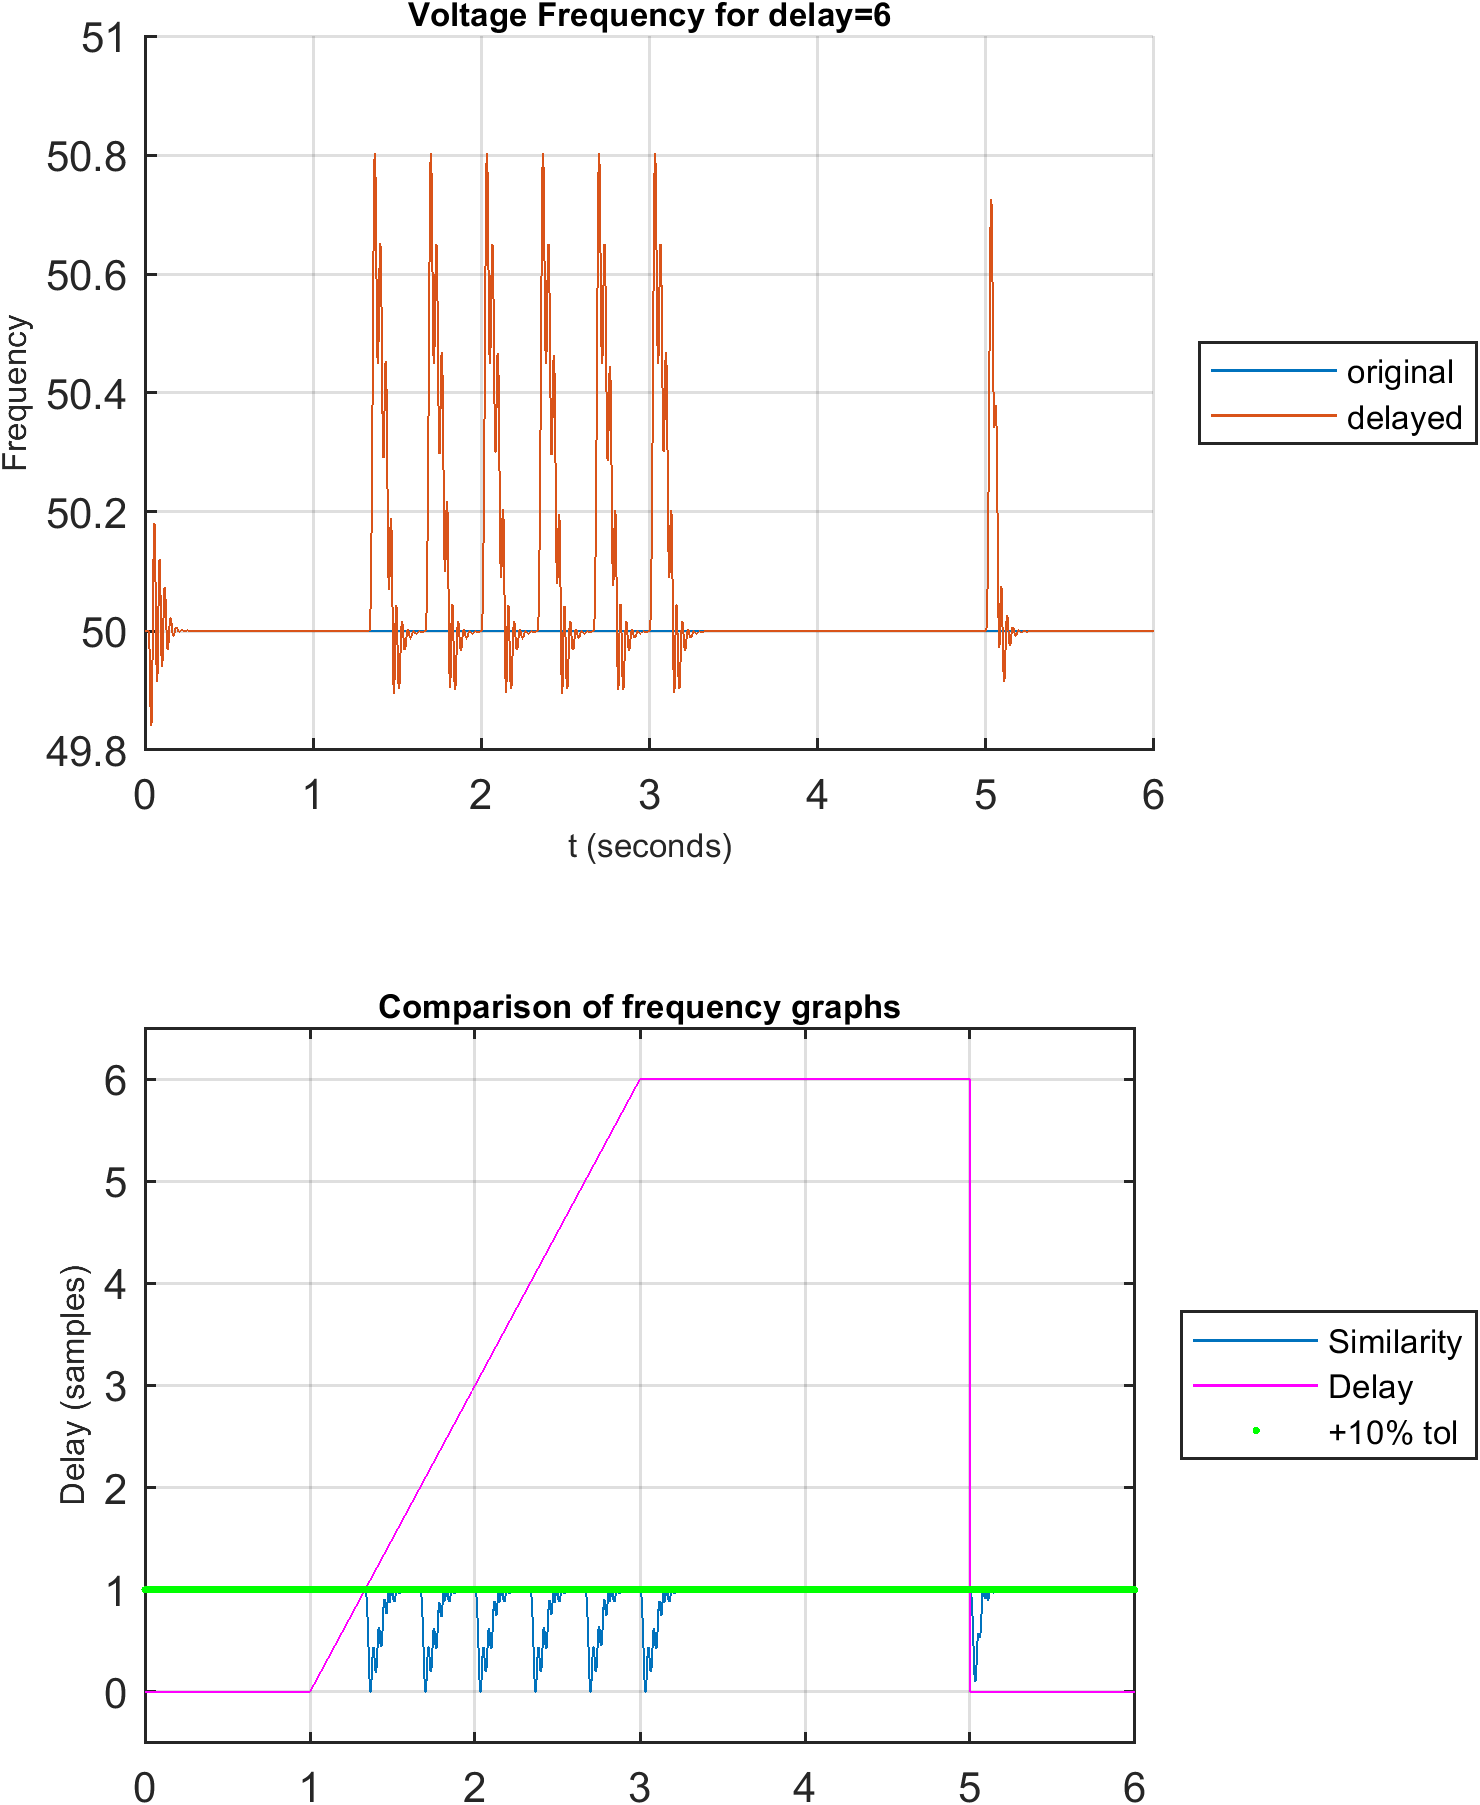
\includegraphics[width=\textwidth]{\locateResults/Frequency.png}    
         %\caption{Frequency Output}
         \label{fig:PMUsim-Con6Freq}
        \caption{Ascending delay of 6: Frequency component output}
 
\end{figure}


